% GNUPLOT: LaTeX picture with Postscript
\begingroup
  \makeatletter
  \providecommand\color[2][]{%
    \GenericError{(gnuplot) \space\space\space\@spaces}{%
      Package color not loaded in conjunction with
      terminal option `colourtext'%
    }{See the gnuplot documentation for explanation.%
    }{Either use 'blacktext' in gnuplot or load the package
      color.sty in LaTeX.}%
    \renewcommand\color[2][]{}%
  }%
  \providecommand\includegraphics[2][]{%
    \GenericError{(gnuplot) \space\space\space\@spaces}{%
      Package graphicx or graphics not loaded%
    }{See the gnuplot documentation for explanation.%
    }{The gnuplot epslatex terminal needs graphicx.sty or graphics.sty.}%
    \renewcommand\includegraphics[2][]{}%
  }%
  \providecommand\rotatebox[2]{#2}%
  \@ifundefined{ifGPcolor}{%
    \newif\ifGPcolor
    \GPcolortrue
  }{}%
  \@ifundefined{ifGPblacktext}{%
    \newif\ifGPblacktext
    \GPblacktexttrue
  }{}%
  % define a \g@addto@macro without @ in the name:
  \let\gplgaddtomacro\g@addto@macro
  % define empty templates for all commands taking text:
  \gdef\gplbacktext{}%
  \gdef\gplfronttext{}%
  \makeatother
  \ifGPblacktext
    % no textcolor at all
    \def\colorrgb#1{}%
    \def\colorgray#1{}%
  \else
    % gray or color?
    \ifGPcolor
      \def\colorrgb#1{\color[rgb]{#1}}%
      \def\colorgray#1{\color[gray]{#1}}%
      \expandafter\def\csname LTw\endcsname{\color{white}}%
      \expandafter\def\csname LTb\endcsname{\color{black}}%
      \expandafter\def\csname LTa\endcsname{\color{black}}%
      \expandafter\def\csname LT0\endcsname{\color[rgb]{1,0,0}}%
      \expandafter\def\csname LT1\endcsname{\color[rgb]{0,1,0}}%
      \expandafter\def\csname LT2\endcsname{\color[rgb]{0,0,1}}%
      \expandafter\def\csname LT3\endcsname{\color[rgb]{1,0,1}}%
      \expandafter\def\csname LT4\endcsname{\color[rgb]{0,1,1}}%
      \expandafter\def\csname LT5\endcsname{\color[rgb]{1,1,0}}%
      \expandafter\def\csname LT6\endcsname{\color[rgb]{0,0,0}}%
      \expandafter\def\csname LT7\endcsname{\color[rgb]{1,0.3,0}}%
      \expandafter\def\csname LT8\endcsname{\color[rgb]{0.5,0.5,0.5}}%
    \else
      % gray
      \def\colorrgb#1{\color{black}}%
      \def\colorgray#1{\color[gray]{#1}}%
      \expandafter\def\csname LTw\endcsname{\color{white}}%
      \expandafter\def\csname LTb\endcsname{\color{black}}%
      \expandafter\def\csname LTa\endcsname{\color{black}}%
      \expandafter\def\csname LT0\endcsname{\color{black}}%
      \expandafter\def\csname LT1\endcsname{\color{black}}%
      \expandafter\def\csname LT2\endcsname{\color{black}}%
      \expandafter\def\csname LT3\endcsname{\color{black}}%
      \expandafter\def\csname LT4\endcsname{\color{black}}%
      \expandafter\def\csname LT5\endcsname{\color{black}}%
      \expandafter\def\csname LT6\endcsname{\color{black}}%
      \expandafter\def\csname LT7\endcsname{\color{black}}%
      \expandafter\def\csname LT8\endcsname{\color{black}}%
    \fi
  \fi
    \setlength{\unitlength}{0.0500bp}%
    \ifx\gptboxheight\undefined%
      \newlength{\gptboxheight}%
      \newlength{\gptboxwidth}%
      \newsavebox{\gptboxtext}%
    \fi%
    \setlength{\fboxrule}{0.5pt}%
    \setlength{\fboxsep}{1pt}%
\begin{picture}(14400.00,5760.00)%
    \gplgaddtomacro\gplbacktext{%
      \csname LTb\endcsname%%
      \put(618,595){\makebox(0,0)[r]{\strut{}0}}%
      \csname LTb\endcsname%%
      \put(618,1108){\makebox(0,0)[r]{\strut{}0.1}}%
      \csname LTb\endcsname%%
      \put(618,1620){\makebox(0,0)[r]{\strut{}0.2}}%
      \csname LTb\endcsname%%
      \put(618,2133){\makebox(0,0)[r]{\strut{}0.3}}%
      \csname LTb\endcsname%%
      \put(618,2646){\makebox(0,0)[r]{\strut{}0.4}}%
      \csname LTb\endcsname%%
      \put(618,3159){\makebox(0,0)[r]{\strut{}0.5}}%
      \csname LTb\endcsname%%
      \put(618,3671){\makebox(0,0)[r]{\strut{}0.6}}%
      \csname LTb\endcsname%%
      \put(618,4184){\makebox(0,0)[r]{\strut{}0.7}}%
      \csname LTb\endcsname%%
      \put(618,4697){\makebox(0,0)[r]{\strut{}0.8}}%
      \csname LTb\endcsname%%
      \put(618,5209){\makebox(0,0)[r]{\strut{}0.9}}%
      \csname LTb\endcsname%%
      \put(618,5722){\makebox(0,0)[r]{\strut{}1}}%
      \csname LTb\endcsname%%
      \put(720,409){\makebox(0,0){\strut{}\np{0.0}}}%
      \csname LTb\endcsname%%
      \put(1854,409){\makebox(0,0){\strut{}\np{0.5}}}%
      \csname LTb\endcsname%%
      \put(2988,409){\makebox(0,0){\strut{}\np{1.0}}}%
      \csname LTb\endcsname%%
      \put(4122,409){\makebox(0,0){\strut{}\np{1.5}}}%
      \csname LTb\endcsname%%
      \put(5255,409){\makebox(0,0){\strut{}\np{2.0}}}%
      \csname LTb\endcsname%%
      \put(6389,409){\makebox(0,0){\strut{}\np{2.5}}}%
    }%
    \gplgaddtomacro\gplfronttext{%
      \csname LTb\endcsname%%
      \put(126,3158){\rotatebox{-270}{\makebox(0,0){\strut{}Oscillation probability}}}%
      \csname LTb\endcsname%%
      \put(4121,130){\makebox(0,0){\strut{}Length / Energy / \np{e4} (km / GeV)}}%
      \csname LTb\endcsname%%
      \put(4237,5183){\makebox(0,0)[r]{\strut{}$\nu_e \to \nu_\tau$}}%
      \csname LTb\endcsname%%
      \put(4237,5369){\makebox(0,0)[r]{\strut{}$\nu_e \to \nu_\mu$}}%
      \csname LTb\endcsname%%
      \put(4237,5555){\makebox(0,0)[r]{\strut{}$\nu_e \to \nu_e$}}%
    }%
    \gplgaddtomacro\gplbacktext{%
      \csname LTb\endcsname%%
      \put(7421,595){\makebox(0,0)[r]{\strut{}}}%
      \csname LTb\endcsname%%
      \put(7421,1108){\makebox(0,0)[r]{\strut{}}}%
      \csname LTb\endcsname%%
      \put(7421,1620){\makebox(0,0)[r]{\strut{}}}%
      \csname LTb\endcsname%%
      \put(7421,2133){\makebox(0,0)[r]{\strut{}}}%
      \csname LTb\endcsname%%
      \put(7421,2646){\makebox(0,0)[r]{\strut{}}}%
      \csname LTb\endcsname%%
      \put(7421,3159){\makebox(0,0)[r]{\strut{}}}%
      \csname LTb\endcsname%%
      \put(7421,3671){\makebox(0,0)[r]{\strut{}}}%
      \csname LTb\endcsname%%
      \put(7421,4184){\makebox(0,0)[r]{\strut{}}}%
      \csname LTb\endcsname%%
      \put(7421,4697){\makebox(0,0)[r]{\strut{}}}%
      \csname LTb\endcsname%%
      \put(7421,5209){\makebox(0,0)[r]{\strut{}}}%
      \csname LTb\endcsname%%
      \put(7421,5722){\makebox(0,0)[r]{\strut{}}}%
      \csname LTb\endcsname%%
      \put(7523,409){\makebox(0,0){\strut{}\np{0.0}}}%
      \csname LTb\endcsname%%
      \put(8657,409){\makebox(0,0){\strut{}\np{0.5}}}%
      \csname LTb\endcsname%%
      \put(9791,409){\makebox(0,0){\strut{}\np{1.0}}}%
      \csname LTb\endcsname%%
      \put(10925,409){\makebox(0,0){\strut{}\np{1.5}}}%
      \csname LTb\endcsname%%
      \put(12059,409){\makebox(0,0){\strut{}\np{2.0}}}%
      \csname LTb\endcsname%%
      \put(13193,409){\makebox(0,0){\strut{}\np{2.5}}}%
      \csname LTb\endcsname%%
      \put(14327,409){\makebox(0,0){\strut{}\np{3.0}}}%
    }%
    \gplgaddtomacro\gplfronttext{%
      \csname LTb\endcsname%%
      \put(7421,3158){\rotatebox{-270}{\makebox(0,0){\strut{}}}}%
      \csname LTb\endcsname%%
      \put(10925,130){\makebox(0,0){\strut{}Length / Energy / \np{e4} (km / GeV)}}%
      \csname LTb\endcsname%%
      \put(11041,5183){\makebox(0,0)[r]{\strut{}$\nu_\mu \to \nu_\tau$}}%
      \csname LTb\endcsname%%
      \put(11041,5369){\makebox(0,0)[r]{\strut{}$\nu_\mu \to \nu_\mu$}}%
      \csname LTb\endcsname%%
      \put(11041,5555){\makebox(0,0)[r]{\strut{}$\nu_\mu \to \nu_e$}}%
    }%
    \gplbacktext
    \put(0,0){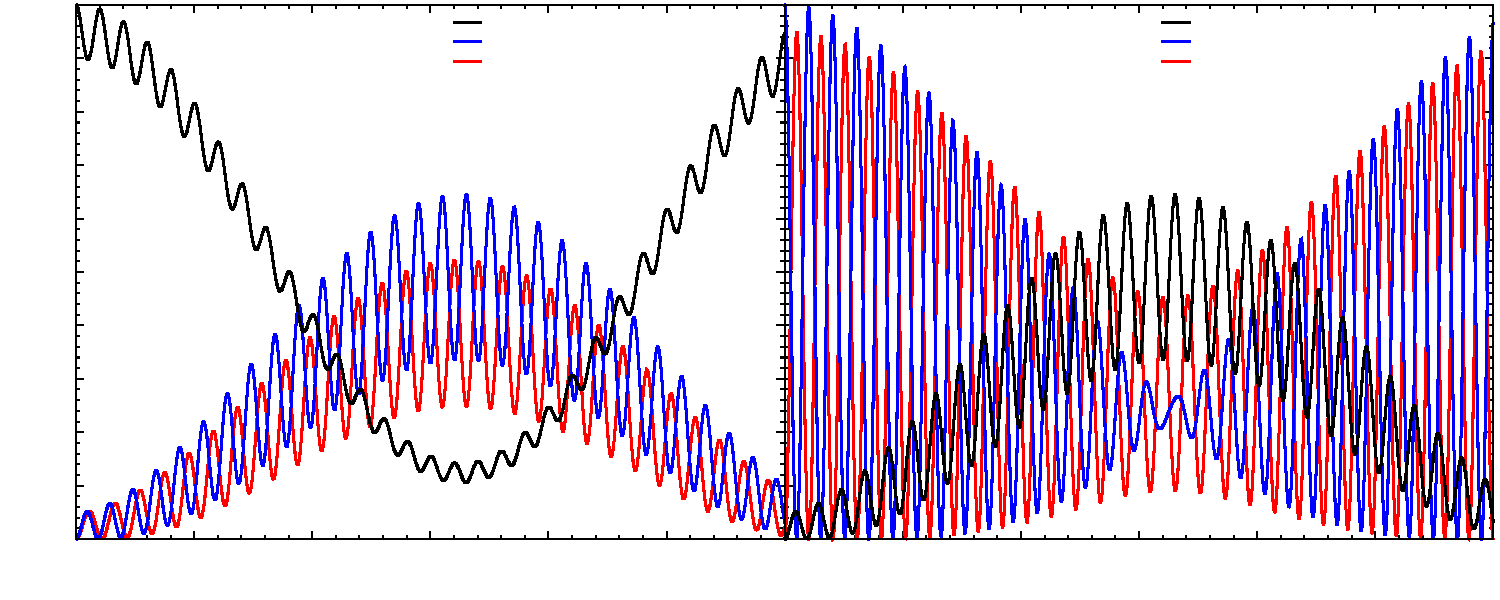
\includegraphics{pics/oscillatorybehave}}%
    \gplfronttext
  \end{picture}%
\endgroup
